\documentclass[sigconf]{acmart}

% --- ACM course-paper setup: keep running heads, drop copyright/ref block/folios ---
\settopmatter{printacmref=false, printccs=false, printfolios=false}
\setcopyright{none}
\renewcommand\footnotetextcopyrightpermission[1]{}
\acmConference[ECS 111]{ECS 111: Machine Learning}{Spring 2026}{University of California, Davis}
\acmDOI{}
\acmISBN{}

\usepackage{booktabs}
\usepackage{graphicx}
\usepackage{cuted}   % full-width inline (non-floating) bands for Figures 5 and 6
\graphicspath{{figures/}}
\setlength{\emergencystretch}{2em}  % absorb minor over-wide lines without changing text

% keep short floats from being banished to their own page
\renewcommand{\textfraction}{0.08}
\renewcommand{\topfraction}{0.92}
\renewcommand{\bottomfraction}{0.92}
\renewcommand{\floatpagefraction}{0.85}

% Shared affiliation for all five authors.
\newcommand{\ucd}{%
  \affiliation{%
    \institution{University of California, Davis}
    \city{Davis}\state{CA}\country{USA}}}

\begin{document}

\title{Chain-of-Thought Prompting versus Fine-Tuning for Table Reasoning in Small Language Models}

\author{Adisesh Venkatesh}\ucd \email{adivenkatesh@ucdavis.edu}
\author{Amar Thota}\ucd \email{asthota@ucdavis.edu}
\author{Nikhil Karthikeyan}\ucd \email{nkarthikeyan@ucdavis.edu}
\author{Sanjay Manivasagam}\ucd \email{sanmanivas@ucdavis.edu}
\author{Anant Madhok}\ucd \email{amadhok@ucdavis.edu}

\begin{abstract}
What should one do when a small, free language model exists: Should one invest effort into chain-of-thought (CoT) prompting or into supervised fine-tuning to enable the language model to answer questions about tables? We perform a controlled comparison between FLAN-T5-base (250M), FLAN-T5-large (780M) models on WikiTableQuestions (WTQ) and a held-out generalization test on TabFact, with two random seeds per model, and numbers reported in the results file are not hand-typed. Our results were negative and consistent: none of our methods outperform a plain zero-shot baseline. While few-shot CoT doubled the exact match compared to plain CoT (0.015 base vs. 0.052 few-shot), and lighter fine-tuning of the base model (0.157 answers-only vs. 0.121 with reasoning traces) still struggled to beat the plain CoT baseline (0.171 base), the strongest system overall was FLAN-T5-large prompted with no examples, which achieved 0.241 exact match. The fine-tuned models do not transfer at all on the out-of-distribution TabFact transfer, as their ability to output a gradeable true/false token is almost nonexistent (0.5\% mappable outputs), and hence their accuracy on out-of-distribution TabFact comes from the output-format collapse at transfer time due to distribution shift, not from table-fact reasoning. We argue that the reason for CoT degradation is a format effect: small models reason in prose but the strict exact match reward is purely the cell, and we statistically confirm the prompting-vs-fine-tuning gap is not an artefact of the head-lines (McNemar, $p<10^{-13}$). We believe the very best model to choose, at this scale and compute budget, is the largest one that can be prompted in a straightforward manner, using careful output formatting, as opposed to using CoT or a quick fine-tune.
\end{abstract}

\maketitle

\section{Introduction}
In real life, data exists in different rows and columns: sports outcomes, financial reports, medical records and government statistics are all examples of data found in tables. The language model is of little value if it fails to read a table reliably, even if it is very good in free text. However, table question answering is a surprisingly difficult task: it is a multi-step pipeline, with each step being: understand the question; find the relevant cells; select the correct operation (filter, count, compare, sort); and output an answer in a desired format, confident if the answer is incorrect.

There are two simple remedies. The Chain of thought (CoT) prompting method instructs the model to think step-by-step while inference, which does not involve any training. Supervised fine-tuning, on the other hand, fine-tunes the model's weights on question/answer pairs. There is little published evidence for either of these, and most of that is very large and expensive. Wei et al. [5] found that CoT is a emergent benefit of scale and that smaller models are only getting a tiny bit of the fine-tuning benefits; most evidence of fine-tuning relies on compute that a student/hobbyist using a free Colab GPU would not have, anyway.

This paper investigates this under-explored regime directly---both methods, on small models that can be run by anyone for free, under a strict budget (a single free Colab T4, under two hours per model condition). We pose a penetrating, practical question: when you can't purchase a 100B-parameter model, which lever helps table reasoning more, prompting or fine-tuning, and where does each one fail? We contribute:
\begin{enumerate}
  \item A controlled comparison of zero-shot, two CoT prompt styles, and two fine-tuning recipes on the same small models (FLAN-T5-base and -large), with two seeds and reproducible seeded data slices.
  \item A cross-dataset generalization test (train on WTQ, evaluate on TabFact with zero TabFact training) that isolates transfer from memorization.
  \item An honest decomposition of the TabFact transfer result that separates reasoning failure from output-format failure --- the distinction that makes the near-zero numbers interpretable.
  \item A failure analysis (error-type breakdown, chain-quality rating with inter-rater agreement, and a paired significance test) and a full provenance discipline in which every reported number is regenerated from a result file by a script that fails loudly on any unmapped figure.
\end{enumerate}
Our findings are negative, and we report them as such: no condition beat the plain baseline. We argue this is itself a useful, reproducible result for the small-model regime, and we explain the mechanisms behind it.

\section{Related Work}
\textbf{Chain-of-thought prompting.} Recently, CoT prompting was introduced by Wei et al. [5] who demonstrated that this prompting encourages reasoning in models with over about 100B parameters, explicitly stating that smaller models sufficiently benefit from it, if at all, and could be adversely affected. Since then, several works have led to higher performance for large models: self-consistency [4] compares multiple sampled chains, and tree-of-thoughts [7] goes through reasoning branches, but they do not explicitly account for inference cost and/or do not focus on large models or on tables, respectively. Weevaluate the small-model bound-ary that Wei et al. identified in their work, on a structured-input task, under a tight compute cap.

Ask questions about the tables and check that they are correct. We present compositional QA for semi-structured tables: filtering, aggregation, comparison and multi-hop table QA (in WikiTableQuestions [3]). In TabFact [1] the concept of table understanding was posed as binary fact verifiers (true/false over a statement and over a table). In TAPAS [2] intermediate steps are not given in the learning algorithm and a table specialized encoder is trained under weak supervision. The most similar previous task to the one we have framed, UnifiedSKG [6] unified many structured-knowledge tasks under a text-to-text interface but is not quantitatively different from ours in terms of prompting vs. fine-tuning framed as a controlled experiment, nor is it encumbered by strict free-tier compute limits.

This situation of the work. Each component (CoT, table QA, seq2seq fine-tuning) is given. The specific combination is not a controlled prompting-vs-fine-tuning comparison, 250M--780M scale, WTQ and TabFact datasets, free Colab budget, cross-dataset transfer test and an error-type breakdown. Our gap -- empirical evidence for practitioners who cannot scale.

\section{Methodology}
\subsection{Models}
We use the FLAN-T5 family: FLAN-T5-base (250M parameters) and FLAN-T5-large (780M). The base model is both prompted and fine-tuned; the large model is prompt-only, because fine-tuning it exhausts the 16 GB of a free Colab T4. FLAN-T5-small (80M) is used only for a fast end-to-end smoke check, never for reported numbers. All generation is greedy (\texttt{do\_sample=False}, \texttt{num\_beams=1}), making decoding deterministic.

\subsection{Datasets}
Both datasets require no account/API key to load from the HuggingFace Hub. We use content-identical parquet mirrors, since \textgreater{}=~4.0 of the datasets pulled script-by-script wikitablequestions and tab\_fact, no longer loading. The pool of examples in WTQ is compiled from lighteval/wikitablequestions, which is just one 18,486-example pool of examples of which we carve a fixed, seeded disjoint partition of train/eval examples, never mixing and matching. The data in TabFact is derived from target-benchmark/tabfact-queries and joined with tabfact-corpus on the table\_id. Each table is store in a text format, with column headers first and then data for each row in rows separated by a bar, the token limit for which is small. The main train and test task is the WTQ, while TabFact is only available for evaluation purposes, does not participate in the training itself and thus measures the transfer of the fine-tuned model's performance rather than mere memorization.

\subsection{Conditions}
We evaluate six conditions, ordered so earlier ones stand alone:

\begin{table*}[t]
\centering
{\normalsize\textbf{Experimental conditions.}}\par\smallskip
\setlength{\tabcolsep}{6pt}\small
\begin{tabular}{@{}llllp{0.40\textwidth}@{}}
\toprule
\# & Condition & Model(s) & Training & Description \\
\midrule
C0 & Baseline & base + large & none & Question + serialized table, no examples. The floor. \\
CA-plain & CoT, plain & base + large & none & Six hand-written exemplars with free-paragraph reasoning prepended. \\
CA-struct & CoT, structured & base + large & none & Same six exemplars, reasoning as a fixed step template. \\
CB & Fine-tune, answers-only & base & yes & Target = final answer only (standard fine-tuning). \\
CC & Fine-tune, + reasoning traces & base & yes & Target = a rule-generated reasoning chain ending in the answer. \\
CG & Generalization & CB \& CC models, + base floor & none & The fine-tuned (and untrained-base) models evaluated on TabFact, zero TabFact training. \\
\bottomrule
\end{tabular}
\end{table*}

The two CoT styles let us separate whether reasoning demonstrations help from whether their format matters. The reasoning traces in CC are produced by rule-based templates that emit a chain only when the derivation is unambiguous and otherwise fall back to the plain answer, so a wrong chain never enters training; coverage was 3,740 of 8,000 training rows (46.8\%) for both seeds.

\subsection{Training}
Two recipes are used to fine-tune: just one recipe for each model (CB and CC), and using a batch size 8 and gradient accumulation 4 (effective batch 32) to keep the comparison fair, as well as three epochs, on a T4. The only difference between CB and CC is the target Text, which is the students' writing assignment for the fall semester. Mean $\pm$ standard deviation are given for the two conditions (seeds 13 and 42).

\subsection{Evaluation and Statistics}
The official run evaluates on 1,000 examples for the baseline, fine-tuning, and TabFact conditions, and on 500 for the slower CoT conditions; the training pool is 8,000 examples. Metrics:
\begin{itemize}
  \item Exact match (EM) --- primary WTQ metric; predictions and golds are normalized (lowercased, punctuation removed) before comparison.
  \item Token-level F1 --- partial credit where EM is too strict (lists, ranges).
  \item Classification accuracy --- TabFact; the model's free-form output is mapped to true/false by a keyword verbalizer (true/\allowbreak yes/\allowbreak entail/\allowbreak supported/\allowbreak correct $\rightarrow$ true; false/\allowbreak no/\allowbreak refut/\allowbreak contradict/\allowbreak incorrect $\rightarrow$ false), and outputs matching neither (or both) are unmappable and scored wrong.
  \item Error-type breakdown --- every wrong WTQ answer is labeled lookup, aggregation, or multi-hop from question cues.
  \item Chain quality --- 100 sampled CoT chains scored 0/1/2 by two independent rubrics (one strict, one lenient), with Cohen's $\kappa$ for inter-rater agreement.
  \item Compute --- inference seconds per example.
\end{itemize}
For the headline comparison (best CoT vs. best fine-tune on the base model), we run McNemar's test on paired per-example correctness, using an exact binomial test on the discordant pairs. Provenance is enforced mechanically: \texttt{report\_fill.py} maps each reported figure to a result JSON and \texttt{finalize\_report.py} exits non-zero if any numeric token is left unmapped, so no number in this paper is hand-typed.

\section{Experiments and Results}
\subsection{Main task: WikiTableQuestions}
Table~\ref{tab:wtq} reports exact match and token-F1 for every WTQ condition, as mean $\pm$ std over seeds 13 and 42.

\begin{table}[t]
\centering
\caption{WikiTableQuestions---exact match and token-F1 (mean $\pm$ std, 2 seeds).}
\label{tab:wtq}
\small
\begin{tabular}{@{}llcc@{}}
\toprule
Condition & Model & Exact Match & Token-F1 \\
\midrule
Baseline & base & $0.171 \pm 0.011$ & $0.204 \pm 0.011$ \\
Baseline & large & $0.241 \pm 0.009$ & $0.279 \pm 0.011$ \\
CoT, plain & base & $0.015 \pm 0.001$ & $0.062 \pm 0.001$ \\
CoT, plain & large & $0.052 \pm 0.008$ & $0.099 \pm 0.007$ \\
CoT, structured & base & $0.019 \pm 0.003$ & $0.059 \pm 0.001$ \\
CoT, structured & large & $0.147 \pm 0.015$ & $0.197 \pm 0.011$ \\
Fine-tune, answers & base & $0.157 \pm 0.002$ & $0.207 \pm 0.006$ \\
Fine-tune, traces & base & $0.121 \pm 0.009$ & $0.158 \pm 0.012$ \\
\bottomrule
\end{tabular}
\end{table}

\begin{figure}[tb]
\centering
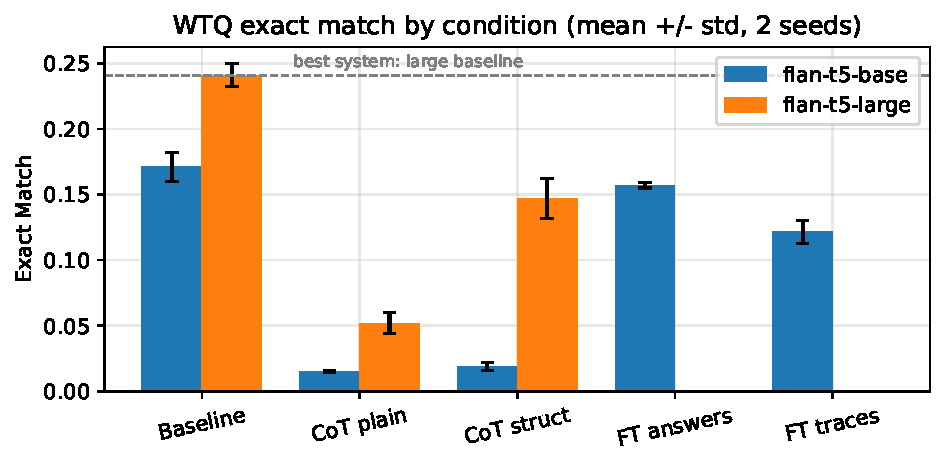
\includegraphics[width=\columnwidth]{fig1.pdf}
\Description{Grouped bar chart of WikiTableQuestions exact match for each condition on the base and large models, with the large-model baseline highest.}
\caption{WTQ exact match by condition and model; error bars are std over seeds 13 and 42. The dashed line marks the best system, the large-model baseline at 0.241.}
\label{fig:wtq-em}
\end{figure}

Three results are noteworthy. The plain baseline is the most successful at all comparisons. The highest score in the study is obtained by a method which is classification true while the baseline methods are not classification true with base model FLAN-T5 with no example: 0.241 EM. Exact match is very sensitive to CoT. Plain CoT reduces the large model to 0.052, an improvement of over 4$\times$ from the baseline large model, and the base model to 0.015, over 4.6$\times$ improvement from the large model baseline. Less destructive on the large model (0.147), but significantly below their base model (0.241) level, and no better than plain CoT (0.019) on base. Neither does fine-tuning do: Fine-tuning with answers only results in 0.157, and fine-tuning with reasoning traces results in 0.121.

\begin{figure}[tb]
\centering
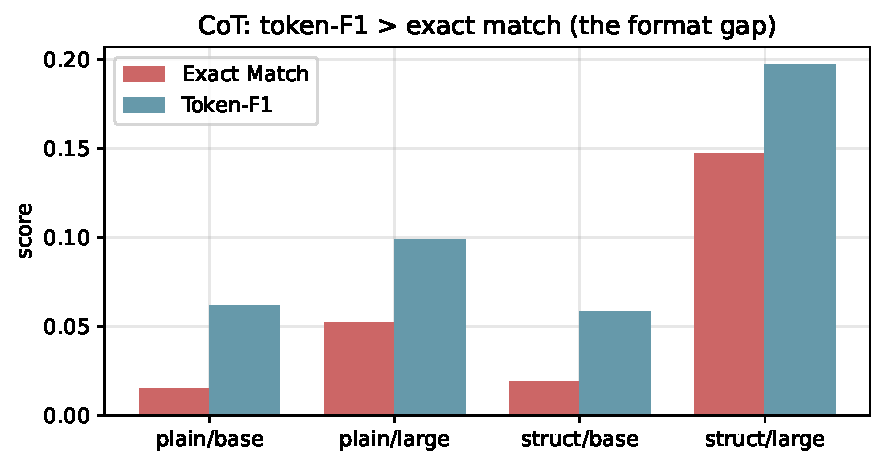
\includegraphics[width=\columnwidth]{fig2.pdf}
\Description{Paired bar chart showing token-F1 exceeding exact match for each CoT condition and model.}
\caption{On the CoT conditions token-F1 stays above exact match: the model keeps relevant content but not the bare cell value that exact match rewards.}
\label{fig:cot-gap}
\end{figure}

\subsection{Generalization: TabFact transfer}
The test is fair because the TabFact eval explicitly asks for a true or false response and scores the maps based on the free-form output via the verbalizer above. The gold split of 1000 is 551 false / 449 true, resulting in a majority class floor of 0.551. Here we report four quantities per model, as raw accuracy is not telling us the story:

\begin{table*}[t]
\centering
\caption{TabFact transfer (zero TabFact training, pooled over 2 seeds, $n = 2000$). Floor $= 0.551$.}
\label{tab:tabfact}
\small
\begin{tabular}{@{}lcccc@{}}
\toprule
Model & Accuracy & Mappable outputs & Unmappable & Accuracy $\mid$ mappable \\
\midrule
Untrained base (floor) & $0.043 \pm 0.000$ & 170 / 2000 & 0.915 & 0.506 ($n = 170$) \\
Fine-tune, answers & $0.003 \pm 0.001$ & 11 / 2000 & 0.995 & 0.455 ($n = 11$) \\
Fine-tune, traces & $0.002 \pm 0.001$ & 13 / 2000 & 0.994 & 0.308 ($n = 13$) \\
\bottomrule
\end{tabular}
\end{table*}

\begin{figure*}[t]
\centering
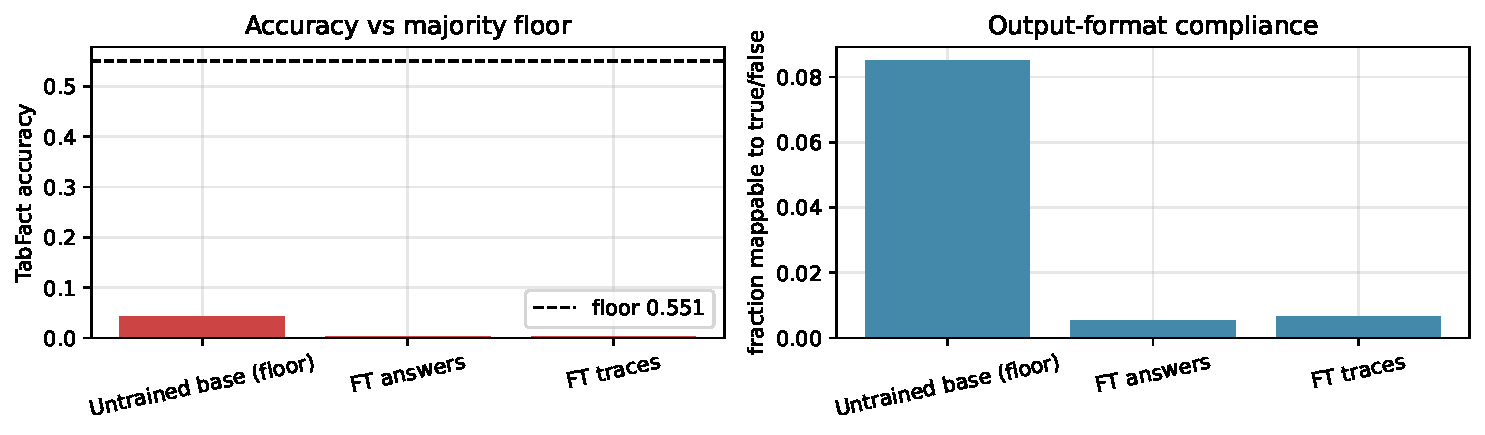
\includegraphics[width=\textwidth]{fig3.pdf}
\Description{Two panel bar chart: left panel TabFact accuracy far below the 0.551 floor for all three models; right panel the fraction of outputs mappable to true or false.}
\caption{TabFact transfer with zero TabFact training. Left: accuracy against the 0.551 majority-class floor. Right: the fraction of outputs the verbalizer can map to true or false.}
\label{fig:tabfact}
\end{figure*}

These accuracies (between 0.1 and 4.3\%) are far short of the 60\% goal specified in our proposal and the 0.551 majority floor. This is because of decomposition: there almost never is a gradeable true-falseness token that is emitted by the models. In the case of the untrained base, it gives a mappable answer only 8.5\% of its time, in the case of the WTQ-fine-tuned version it only 0.5\% of the time (with only the literal token in the output of the answers model, which it emitted 0 153 times in one seed). More importantly, if the untrained base does answer in-format, it is correct 0.506 of the time (chance). The conditional rates are not easily interpretable and are based on 11 and 13 examples. That is an output format collapse under distribution shift, not anti-correlation with truth: the models were not trained to see the facts, and the simple addition of more examples of the aforementioned distribution -- with them being examples of well-known facts -- actually worsened the format mismatch problem.

\subsection{Error analysis}
All incorrect WTQ responses are identified with a reasoning type. Table~\ref{tab:errors} shows the percentages of each type of error within the set of incorrect answers, combined over the two seeds.

\begin{table}[t]
\centering
\caption{WTQ error-type share among wrong answers (pooled, 2 seeds).}
\label{tab:errors}
\small
\begin{tabular}{@{}lccc@{}}
\toprule
Condition (model) & Lookup & Aggregation & Multi-hop \\
\midrule
Baseline (base) & 26\% & 61\% & 13\% \\
Baseline (large) & 24\% & 64\% & 12\% \\
CoT plain (base) & 31\% & 57\% & 13\% \\
CoT structured (large) & 28\% & 60\% & 13\% \\
Fine-tune answers (base) & 29\% & 57\% & 14\% \\
Fine-tune traces (base) & 30\% & 55\% & 15\% \\
\bottomrule
\end{tabular}
\end{table}

\begin{figure*}[t]
\centering
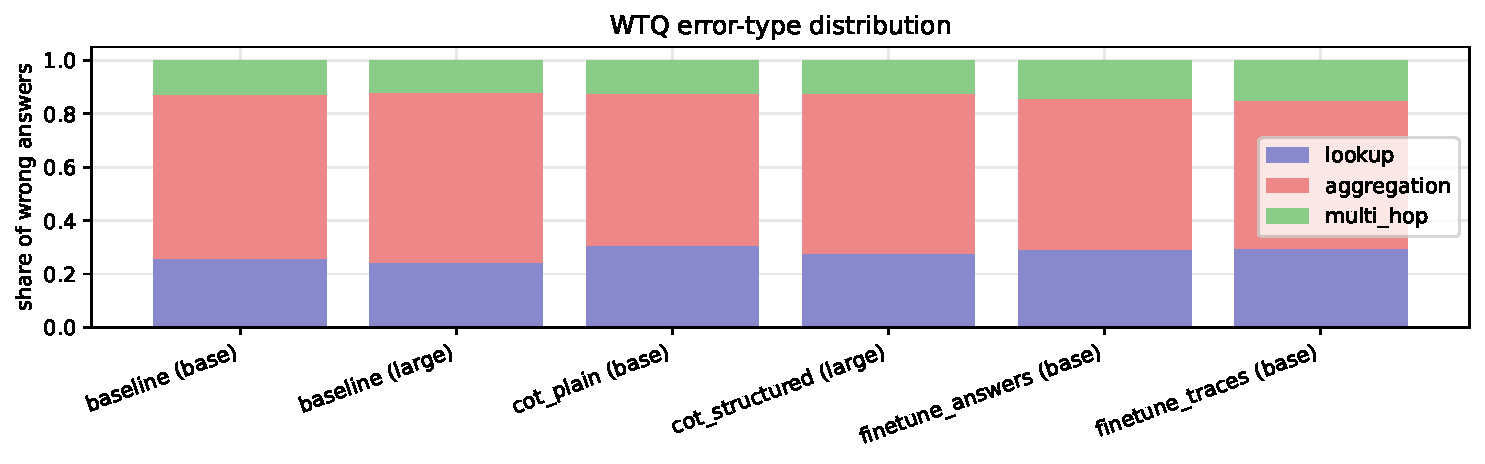
\includegraphics[width=\textwidth]{fig4.pdf}
\Description{Stacked bar chart of lookup, aggregation, and multi-hop error shares across the six conditions, with aggregation dominant everywhere.}
\caption{Share of each error type among wrong WTQ answers, pooled over both seeds.}
\label{fig:errdist}
\end{figure*}

The most common error types are aggregation questions (55--64\% of all errors), followed a long way behind by lookups, and multi-hop steady is near 8\%. The error mix doesn't change much across conditions: CoT didn't affect the model's failure to model what it fails at, but rather simply reduced the number of answers the model gets right. The reasoning-traces fine-tune is the most obvious downside: it was engineered to eliminate reasoning errors, but its share of aggregated answers (55\%) is about the same as the answers-only model (57\%) and its multi-hop share actually increased, as the chains got longer but the operations remained the same.

\subsection{Chain quality}
Two rubrics were used, one strict (which only gave full credit for a chain that names a concrete table operation and leads to the gold answer), and one lenient (which gave credit for any multi-step chain that leads to an answer).Two rubrics, one strict (full credit only for a chain that names a concrete table operation and reaches the gold answer) and one lenient (credit for any multi-step chain that reaches an answer), were used. The mean scores were near the floor: 0.11 (strict) and 0.15 (lenient); and the two rubrics agreed at Cohen's $\kappa = 0.784$ (substantial). By both standards the chains are mostly empty, or even degenerate, and this is reinforced by the presence of a strong $\kappa$ that makes this read unlikely to be one of the quirks in the standard.

\subsection{Significance}
It is the headline comparison that gives $p < 10^{-13}$ ($p = 2.2\times10^{-14}$, seed 13) when we are performing the comparison on the base model (McNemar's exact test on per-example correctness). This is not a noise issue with the seeds, this is an issue of a gap: Fine tuning beats prompting on base model. There is no negative impact on the headline, they both remain beaten by the plain baseline.

\begin{strip}
{\centering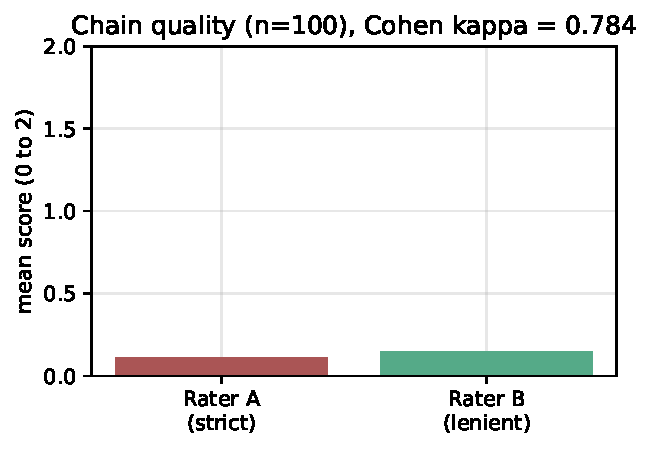
\includegraphics[width=0.5\textwidth]{fig5.pdf}\par}
\smallskip
\refstepcounter{figure}\label{fig:chainq}%
{\small\textbf{Figure~\thefigure:} Chain-quality means under the strict and lenient rubrics ($n=100$); the two raters agree at Cohen's $\kappa = 0.784$.\par}
\end{strip}

\subsection{Compute}
The number of seconds needed to infer the answer (seconds per example) follows the length of the prompt as expected. The fine-tuned base inference is the fastest of all with 0.091 s (answers), since it produces shorter answers, whereas CoT is 2--3.5$\times$ slower (0.290--0.308 s base, 0.715--0.718 s large); and baseline inference is the cheapest (0.126 s base, 0.200 s large). All conditions done in under 2hrs per condition on free T4.

\begin{strip}
{\centering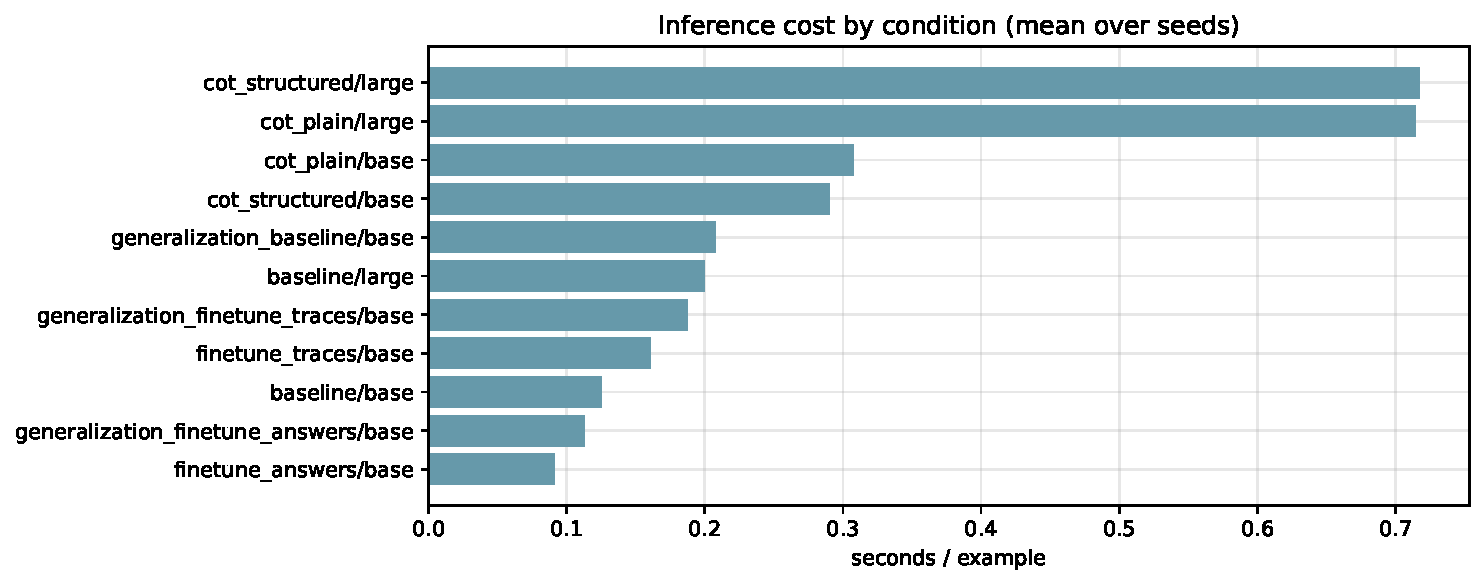
\includegraphics[width=\textwidth]{fig6.pdf}\par}
\smallskip
\refstepcounter{figure}\label{fig:compute}%
{\small\textbf{Figure~\thefigure:} Inference cost in seconds per example by condition, mean over seeds.\par}
\end{strip}

\section{Discussion and Analysis}
Why CoT hurts. The damage is not a thinking damage, it's a format damage. Originally, when matching was simply to receive an output from the bare cell, FLAN-T5 was not even capable of producing one, a cell with the text ``The total number of senators\ldots{} is 130. These differences are also found in Token-F1 (e.g., Token 97.5 vs. F1 0.197) -- which also allows for some points to be earned -- and are more pronounced than in EM (e.g., structured-large F1 0.197 vs. EM 0.147) indicating that more content of the answer is held, but there is less similarity in its surface form. This mirrors what Wei et. al. discovered: models at this size don't benefit that much from CoT; we'd like to add to this case, that strict-match table QA matters negatively--format mismatch, indeed.

The reason for not transferring fine-tuning. Fine-tuning on WTQ adds fine-tuning, which yields succinct answers with facts. That's just the opposite of what TabFact requires: a true or false token. The fine-tuned models thus produce output similar to that produced by the verbalizer WTQ on TabFact which cannot be covered by the verbalizer, leading to 0.5\% coverage. That does not help the reasoning-traces variant either: those of the EM and the TabFact variants performed worse in both the WTQ EA and the TabFact transfer. It seems, therefore, to be best understood in terms of the transfer result as evidence for what might be called the fine tuning analogue of the prompting format effect: Format lock-in.

The lessons the practitioner should take away from. The model one can choose is the most leveraged model without sacrificing any accuracy; a few-shot CoT model and a quick fine-tune are models which sacrifice accuracy for leverage here. The simplest baseline will probably provide the most reliable indication in our research.

Constraints and potential weaknesses on validity. (1) Eval is not the test set, but a 1000-example slice to respect the budget to be under 500 on CoT; the standard deviation is small across two seeds so the slice seems to be consistent, but it is a sampled slice. Large models have been fine-tuned on a T4 only on the base mode, so there is no way of knowing what fine-tuning behavior this large model will exhibit on a T4. The breakdown provided is approximate as it is based on the error-type labels (question-cue based). (4) The trace generator only generates unambiguous derivations (46.8\% of the rows) and CC relies on plain answers for the rest that might eliminate any trace effect. The TabFact accuracies are the format-compliance scores in the distribution shift setting, as opposed to reasoning scores; and for this reason we report the decomposition.

\section{Conclusion}
At this size, we wondered if reading tables is better supported by chain-of-thought prompting, versus by supervised fine-tuning of the small model; and indeed, neither. The plain zero-shot baseline on FLAN-T5-large was the best system with 0.241 exact match, while CoT achieved more than a doubling of exact match, light fine-tuning dropped below the baseline, and the accuracy of the WTQ-fine-tuned models was below the majority baseline of 0.551. Both CoT and fine-tuning exacerbate the mismatch, with the mechanisms being two sides of the same issue: small models can handle the content of the tables but are unable to handle the required output format. The obvious takeaway for anyone with a limited compute budget is to explicitly ask the biggest model you have to reason about the problem, rather than doing few-shot reasoning or a quick fine-tune. As a negative result, this is a useful data point for the small-model table-reasoning regime that the literature has largely ignored.

\section*{Contribution Statement}
\begin{itemize}
  \item \textbf{Adisesh Venkatesh} built the shared core library and the baseline condition, wrote the dataset and experimental-setup components, and co-designed and applied the chain-quality rating rubrics.
  \item \textbf{Amar Thota} implemented and ran both chain-of-thought conditions (plain and structured) on both models, led the hand-written CoT exemplars, and assembled the slide deck.
  \item \textbf{Nikhil Karthikeyan} built the seq2seq training harness, ran the answers-only fine-tuning across both seeds, and co-designed and applied the chain-quality rating rubrics.
  \item \textbf{Anant Madhok} built the rule-based reasoning-trace generator and ran the reasoning-traces fine-tuning across both seeds.
  \item \textbf{Sanjay Manivasagam} led and coordinated the project, ran the TabFact generalization test, and produced the error analysis, the statistical tests (McNemar, Cohen's $\kappa$, mean/std), the results tables and plots, and the merged report.
\end{itemize}

\section*{References}
\begingroup
\small
\setlength{\parindent}{-1.2em}
\setlength{\leftskip}{1.2em}
\setlength{\parskip}{2pt}
[1] Chen, W., Wang, H., Chen, J., Zhang, Y., Wang, H., Li, S., Zhou, X., \& Wang, W. Y. (2020). \textit{TabFact: A Large-scale Dataset for Table-based Fact Verification.} ICLR 2020.\par
[2] Herzig, J., Nowak, P. K., M\"uller, T., Piccinno, F., \& Eisenschlos, J. M. (2020). \textit{TAPAS: Weakly Supervised Table Parsing via Pre-training.} ACL 2020.\par
[3] Pasupat, P., \& Liang, P. (2015). \textit{Compositional Semantic Parsing on Semi-Structured Tables.} ACL 2015.\par
[4] Wang, X., Wei, J., Schuurmans, D., Le, Q., Chi, E., Narang, S., Chowdhery, A., \& Zhou, D. (2023). \textit{Self-Consistency Improves Chain of Thought Reasoning in Language Models.} ICLR 2023.\par
[5] Wei, J., Wang, X., Schuurmans, D., Bosma, M., Ichter, B., Xia, F., Chi, E., Le, Q., \& Zhou, D. (2022). \textit{Chain-of-Thought Prompting Elicits Reasoning in Large Language Models.} NeurIPS 2022.\par
[6] Xie, T., Wu, C. H., Shi, P., Zhong, R., Scholak, T., Yasunaga, M., et al. (2022). \textit{UnifiedSKG: Unifying and Multi-Tasking Structured Knowledge Grounding with Text-to-Text Language Models.} EMNLP 2022.\par
[7] Yao, S., Yu, D., Zhao, J., Shafran, I., Griffiths, T. L., Cao, Y., \& Narasimhan, K. (2023). \textit{Tree of Thoughts: Deliberate Problem Solving with Large Language Models.} NeurIPS 2023\par
\endgroup

\end{document}
